\documentclass[12pt]{article}
\usepackage[margin=1in]{geometry}
\setlength{\parindent}{0cm} % don't indent new paragraphs...
%\parskip \psl % ... place a space between paragraphs instead
\usepackage{graphicx, float}
\usepackage[font=small, labelfont=bf]{caption}
%\usepackage[english]{babel}
\usepackage{tikz}
%\usepackage{biblatex}
\usepackage{amsmath}
\usepackage[inline]{enumitem}
%\usepackage{float}
\usetikzlibrary{automata, positioning}
\newcommand{\ignore}[1]{}
\newcommand*{\diff}{\mathrm{d}}
\newcommand{\some}{{\color{red} something}}
\renewcommand{\vec}[1]{\mathbf{#1}}

\floatstyle{plaintop}
\newfloat{algorithm}{thb}{lop}
\floatname{algorithm}{Algorithm}
\newenvironment{alg}{\hrulefill\begin{enumerate}}{\end{enumerate}\hrulefill}

\usepackage[sort&compress,numbers]{natbib}
\bibliographystyle{apsrev4-1}
\usepackage[english]{babel}
\addto\captionsenglish{
    \renewcommand{\contentsname}{Table of Contents}
    \renewcommand{\refname}{References}
}
\usepackage{tocloft}
%\renewcommand{\cftsecleader}{\cftdotfil{\cftdotsep}}


% Commands go here
%%%%%%%%%%%%%%%%%%%%%%%%%%%%%%%%%%%%%%%%%%%%%%%%%%%%%%%%%%%%%%%%%%%%%%%



\renewcommand{\title}{Application of Generalized Renormalization Group Methods to the Square-Well Liquid Near Criticality}

\renewcommand{\author}{Brenden Vischer}

\renewcommand{\date}{02 June 2015}

\renewcommand{\titlepage}{
    {\centering
        \vspace*{4cm}
        
        \title
        
        \vspace{1.5cm}
        
        \author \\
        \text{Advisor: David Roundy}
        
        \vfill
        
        Department of Physics\\
        Oregon State University\\
        \today 
        \newpage}       
}

\begin{document}


\titlepage

\thispagestyle{plain}
\begin{center}
    \Large
    \textbf{Application of Generalized Renormalization Group Methods to the Square-Well Liquid Near Criticality}
    \\or\\
    \textbf{Decomposition of the Critical Square-Well Liquid Into Consitutent Cells}    \\or\\
    \textbf{Free Energy Decomposition of the Critical Square-Well Liquid Using a Renormalization Group Method}
   
    \vspace{0.8cm}
    \large
    A Computational Project
    
    \vspace{0.8cm}
    \textbf{Brenden Vischer}
    
    \vspace{1.2cm}
    \textbf{Abstract}
\end{center}

The free energy of a bulk liquid is a known quantity [cite], near and far from the critical region [cite. true?]. Computing the free energy of a liquid requires lengthy, difficult computations that [something]. These computations generally involve renormalization methods which [do things]. Analytic models using renormalization methods for fluids have been [time scale] developed [cite], but computational models [something]. [something about including all lengths, not knowing what each contributes]. We present a method to determine the free energy contributions of each length scale by exploiting both the behavior of the critical fluid and the periodicity of Monte-Carlo simulations. We further detail a method by which to compute the ``absolute'' free energy, with both the ideal gas free energy and the excess free energy, for the square-well liquid. We determine that the square-well liquid near the critical region is well-characterized by a base cell length of $\sqrt2\sigma$, the side length of an FCC lattice, by establishing liquid-vapor coexistence between scaled temperatures $.5 < T < 1$.   
\clearpage

%%%%%%%%%%%%%%%%%%%%%%%%%%%%%%%%%%%%%%%%%%%%%%%%%%%%%%%%%%%%%%%%%%%%%%%%%%%%%%%%%%%


\tableofcontents
\listoffigures



% Note: include new graphic about probability of move acceptance in Thermo. Int. (see austin thesis)

%%%%%%%%%%%%%%%%%%%%%%%%%%%%%%%%%%%%%%%%%%%%%%%%
%           INTRO                              %
%%%%%%%%%%%%%%%%%%%%%%%%%%%%%%%%%%%%%%%%%%%%%%%%

\section{Introduction}
\subsection{Motivation}
Fluids have long garnered interest\cite{theorysimpleliquids}\cite{theoryofcrits}, particularly among computationally-minded researchers, as an area in which current models are unequipped to robustly predict behavior across multiple regimes. A largely troublesome \cite{white2001global} regime is near the so-called ``critical point'' where liquid and vapor are indistinguishable and, more importantly, large fluctuations of fluid density occur. Most traditional fluid models assume the density across the cell to be nearly constant. As a result, these methods tend to poorly handle these fluctuations near criticality. 
Using the well-established model of the square-well fluid, we seek to determine the applicability of a particular generalized renormalization-group (``GRG'') formalism to find the absolute Helmholtz free energy of systems near criticality.\\

Past efforts to incorporate renormalization group methods into standard Statistical Associating Fluid Theory (``SAFT'') methods have seen success, particularly the treatment offered by Forte et al.~\cite{forte2011application} with the inclusion of a fitted parameter related to the correlation length. GRG's history in fluid simulation has largely been a fitted one - that is, determining a free parameter and then simulating a vast number of cells, varying the parameter each time, to find the most well-suited value for a particular fluid. We present a non-fitted approach that is GRG-minded from the ground up. We exploit the periodicity of Monte-Carlo methods to decompose large cells in the thermodynamic limit into small cells that only allow certain fluctuation wavelengths. We then carefully couple simulations of different ``doubling regimes'', each of which considers a different maximum wavelength of fluctuations, where the number density remains fixed but the volume and number have increased. Summing the difference in absolute Helmholtz free energy $\Delta F^{\text{abs}}$ between doubling regimes will then approximate the absolute free energy of the full cell, including near criticality. Finding absolute free energies is a somewhat challenging problem, but is certainly surmountable with more Monte Carlo. \\
We will begin by outlining the necessary models and assumptions/approximations for this work. We will then detail the algorithms used to compute the quantities with the the discussion on results following. 
\subsection{Hard Sphere}
The hard sphere model approximates monoatomic fluids as having no interactions other than collisions. These spheres exhibit no attraction or repulsion, and consequently each carries kinetic energy $T = 3/2 k_b T$. There is also a harder-to-calculate ``excess'' energy to be considered (which, in fact, contains most of the interesting behavior) which will be discussed further on. The system is defined to have zero total linear momentum, and any collision between two or more spheres is perfectly elastic. For simulation purposes, the system is required to have periodic boundary conditions - that is, when a sphere would classically collide with the wall of the cell it instead breaches the wall and then reappears on the other side of the cell with the same velocity. \\
\ignore{The hard sphere model is incredibly useful; as high temperatures are approached, energy associated with sphere location tends to asymptote for most models [are there any that this isn't true for?] and the kinetic term consequently dominates.}

\subsection{Square-Well Liquid}
The square-well liquid is a ubiquitous approximation that sees extensive use throughout computational fluid research. This simple fluid model consists of hard, immutable spheres that are subject to an intermolecular pair potential - that is, an attractive force between spheres. This model consists of several key parameters: sphere size $\sigma$, well width $\lambda$, and well depth $\epsilon$. These parameters can be fit to model virtually any monoatomic fluid (and some diatomic fluids, such as water). 
 As a hard-sphere model, the spheres are not allowed to overlap. Any arrangement of spheres - hereafter referred to as the ``state'' of the system - that involves either two or more spheres overlapping or a sphere outside the allowed area - ``cell'' - is defined to be invalid. Modifying the radius of the spheres changes the allowed locations in the cell, which in turn affects the partition function of the system. The ``square'' refers to the piecewise intermolecular pair potential $\Phi_{12}$, shown mathematically in Eq. \ref{phi12} and graphically in Figure ~\ref{sw_phi}.

\begin{equation} 
\Phi_{12} = \begin{cases}\infty & |\vec{r}|\leq \sigma\\ -\epsilon & \sigma \leq |\vec{r}| \leq \sigma\lambda\\ 0 & |\vec{r}| > \sigma\lambda \end{cases}
\label{phi12}
\end{equation}

The energy of the fluid is then always an integer multiple of the well depth $\epsilon$. This leads us to choose $\epsilon$ and $\sigma$ as natural scales for the quantities of our simulation. We then define dimensionless temperatures $T/\epsilon$, energies $E/\epsilon$, and distances $r/\sigma$. Moreover, we make the decision to work in geometric units for coding simplicity, setting the Boltzmann constant $k_B$ (as well as any other physical constants) to one.

\begin{figure}
    \centering
    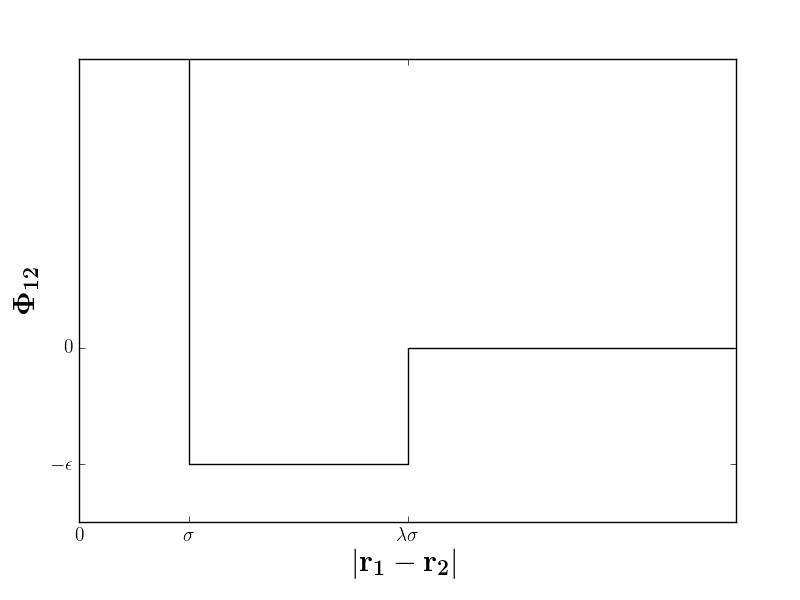
\includegraphics[width=.75\textwidth]{SWF-E.png}
    \caption{Demonstration of Square-Well approximation.}
    \label{sw_phi}
\end{figure}
\subsection{Critical Point} 
The critical point is the temperature and pressure (or any other thermodynamic pairing) on a phase diagram (shown in Figure ~\ref{phase}) where the line between liquid and vapor terminates - liquid and vapor become indistinguishable and are assimilated into the ``fluid'' phase. Many interesting effects occur here, including the well-researched phenomena of critical opalescence. The correlation length, naively interpreted here as the maximum existing wavelength of the density fluctuations within the fluid, diverges to infinity near criticality. As mentioned previously, the diverging of the correlation length invalidates SAFT and many of its variants which assume constant density. 
\begin{figure}
    \centering
    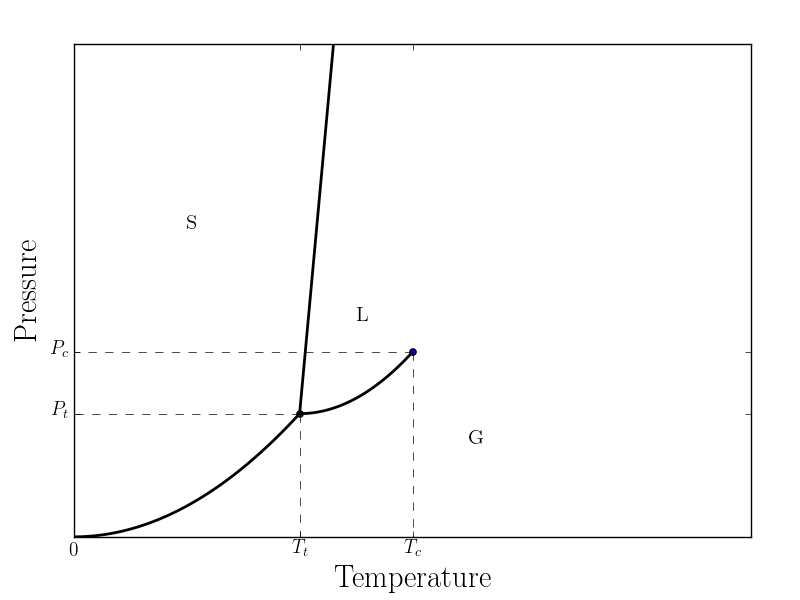
\includegraphics[width=.75\textwidth]{phase.png}
    \caption{Phase transitions of water with critical point and triple point identified.}
    \label{phase}
\end{figure}
\\
The theory of this project is largely predicated upon the behavior of critical systems, namely the phenomena of self-similarity. Non-critical systems exhibit different characteristics when viewed at different length scales. Ever-present small-scale fluctuations in density are relevant, if not dominant, when viewing the system at very small scales, but typically become less important at larger scales and nearly irrelevant near the thermodynamic limit. Near the critical point all wavelengths of fluctuation are present, and so the system looks the same regardless of length scale chosen. This self-similarity allows for the decomposition of the large critical cell to smaller constituent cells. The details of the procedure are more carefully discussed later on.   

\subsection{Free energy}
The free energy we are interested in calculating is the ``absolute'' Helmholtz free energy $F^{\text{abs}}$. The Helmholtz free energy is a Legendre transform of the internal energy $U$:
\begin{align}
    F &= U - TS
    \label{Fdef}
\end{align}
and can be calculated given the ever-pervasive partition function $Z$:
\begin{align}
    F &= -T \ln Z
    \label{FdefSM}
\end{align}
With $F$ calculated, simple partial derivatives yield all other thermodynamic quantities. Though the Gibbs free energy yields the same information, the Helmholtz free energy is particularly useful because of the relationship with entropy:
\ignore{\begin{align}
    S &= \pdd{F}{T}{V}
\end{align}}
\\EQ HERE\\

Equations ~\ref{Fdef} and ~\ref{FdefSM} together bridge classical thermodynamics and statistical mechanics. Due to the nature of this project, we will primarily be concerned with the statistical mechanics definition (that is, Eq. ~\ref{FdefSM}) of the free energy. We are, then, ultimately concerned with determining the partition function for any system we are concerned with. The canonical ensemble partition function can be compactly represented by a summation:
\begin{align}
    Z &= \sum^{\text{energies}}~e^{-\beta E_i}
\end{align}
where $\beta =  T^{-1}$. Of course, it is typically impractical to sum over the individual energies of the system, especially if there are expected degeneracies. Instead we sum over states:
\begin{align}
    Z &= \sum^{\text{states}}~D(E)~e^{-\beta E_i}
\end{align}
where we have now introduced the density of states $D(E)$ which is a simple function that returns the number of states which have a given energy $E$. This introduction is now the focus of calculation - if we can accurately determine the density of states of the system and have knowledge of the available energies, we can calculate the Helmholtz free energy and, from there, any other  \\   
Since $F$ contains a natural log term, we can separate and characterize the individual contributions of kinetic energy (``ideal'') and energy associated with the configuration of the system (``excess'').  
A derivation of the two energy contributions for a monoatomic fluid follows. \\









{\color{red} [This should probably go in an appendix. Further: replace $Z_C$ with $Z_{exc}$; fix the to the N on the $Z_{exc}$ term; include the $N!$ into the ideal term; fix the $V(r_1, r_2, ...)$]}

We begin with the canonical form of the canonical ensemble partition function $Z$:
\begin{align}
    Z &= \sum_i e^{-\beta E_i}
\end{align}
where we sum over individual energies of the system $E_i$. However, this method doesn't account for degeneracies in the system, so instead we sum over the states $s$ (to avoid including the density of states, which is difficult to find for most systems):
\begin{align}
    Z &= \sum_s e^{-\beta E_s}
\end{align} 

Further, the energy of each state is simply the sum of the excess and kinetic energies $V$ and $K$, so

\begin{align}
    E_s &= V_s(\mathbf{r}) + K_s(\mathbf{p})
\end{align}

So now we have 

\begin{align}
    Z &= \sum_S e^{-\beta (V_s(\mathbf{r}) + K_s(\mathbf{p}))}\\
    &= \sum_S e^{-\beta V(\mathbf{r})}~e^{-\beta K(\mathbf{p})}
\end{align} 

Each state is specified by a particular point in phase space (parameterized by $\mathbf{r}$ and $\mathbf{p}$). Even though this phase space is discrete, we can approximate the space as continuous by recognizing that the {\color{red}spacing between individual states is small compared to the total range of the states}, so that the summation becomes an integral:

\begin{align}
    Z &= \int_s~ d\mathbf{r}~ d\mathbf{p} ~e^{-\beta V(\mathbf{r})}~e^{-\beta K(\mathbf{p})}
    %&= \sum_s e^{\beta V(\mathbf{r})}e^{-\beta T(\mathbf{p})}
\end{align} 
However, the above is only partially correct, as it is only for one particle. We can account for multiple particles by requiring that each particle has the same partition function. This is equivalent to integrating $N$ times for $N$ particles:

\begin{align}
    Z &= \int_{s_1} \int_{s_2} ... \int_{s_N} d\mathbf{r_1}~ d\mathbf{p_1} ~d\mathbf{r_2} ~d\mathbf{p_2} ~... ~d\mathbf{r_N}~ d\mathbf{p_N} ~e^{-\beta(V(\mathbf{r_1}) + V(\mathbf{r_2}) ... V(\mathbf{r_N}))}~e^{-\beta(K(\mathbf{p_1}) + K(\mathbf{p_2}) ... K(\mathbf{p_N}))}\\
    &= \left[\int_s d\mathbf{r} ~ d\mathbf{p} ~e^{-\beta V(\mathbf{r})}~e^{-\beta K(\mathbf{p})}\right]^{N}
\end{align}
Additionally, for a proper quantum mechanical treatment we must assume that the particles are indistinguishable which means the above expression over-counts by a factor of $N!$. Our expression for the partition function is then

\begin{align}
    Z &= \frac{1}{N!}\left[\int_s d\mathbf{r} d\mathbf{p} ~e^{-\beta V(\mathbf{r})}~e^{-\beta K(\mathbf{p})}\right]^{N}
\end{align}

Furthermore, we can separate the integrals completely because the exponentials are each attached to only one differential element:

\begin{align}
    Z &= \frac{1}{N!}\left[\int_s d\mathbf{r} ~e^{-\beta V(\mathbf{r})}\right]^{N}\left[\int_s d\mathbf{p} ~e^{-\beta K(\mathbf{p})}\right]^{N}
    \label{Z_full} 
\end{align}
 
We then define the two terms obvious in Eq. \ref{Z_full}, the excess term dependent on the potential energy $V(\mathbf{r})$ and the ideal term dependent on the kinetic energy $K(\mathbf{p})$: 

\begin{align}
    Z &= (Z_{exc})(Z_{id}) \,,
\end{align}
where $Z_{id}$ contains the $N!$ term by convention. The excess term $Z_{exc}$ is system dependent because $V(\mathbf{r})$ is buried inside the integral, but the ideal term is the same for any system where the total energy separates in the preceding fashion. We judiciously decide to leave the excess term alone and work specifically with the ideal term. We then have

\begin{align}
    Z_{id} &=  \frac{1}{N!}\left[\int_s d\mathbf{p} ~e^{-\beta T(\mathbf{p})}\right]^{N}
\end{align}

We begin by imagining a cell of length $L$ and volume $L^3$ in which lives a particle. Then, we quantize the allowed wavelengths of the particle within the cell by defining the wavevector $\mathbf{k}$ as
\begin{align}
    \mathbf{k} &= \frac{2\pi}{L}(n_x\mathbf{\hat{x}} + n_y\mathbf{\hat{y}} + n_z\mathbf{\hat{z}})
\end{align}
It should be noted that this definition of $k$ introduces three-fold degeneracy.\\
Remembering that kinetic energy can be expressed as $T = \frac{\hbar^2 k^2}{2m}$, and using our definition of $\mathbf{k}$:
\begin{align}
    Z_{id} &= \frac{1}{N!}\left[\int_s d\mathbf{p} ~e^{-\beta \frac{\hbar^2 k^2}{2m}}\right]^{N}
    \label{Zt_def}
\end{align}
This unfortunately introduces a mass quantity into the partition function which adds a parameter that needs fitting. [more] 
If we then allow the cell to become very large, then the we can easily see in Eq. \ref{Zt_def} that the spacing between occupants in phase space becomes small, so we can integrate instead $\diff ^3 n$ over all possible values of $n$:
\begin{align}
    Z_{id} &= \frac{1}{N!}\left[\int_0^\infty \diff^3 n ~e^{-\frac{\beta \hbar^2}{2m} \left(\frac{2\pi}{L}(n_x\mathbf{\hat{x}} + n_y\mathbf{\hat{y}} + n_z\mathbf{\hat{z}}\right)^2}\right]^{N} = \frac{1}{N!}\left[\int_0^\infty \diff^3 n ~e^{ \frac{-2\beta \hbar^2\pi^2}{mL^2}(n_x^2 + n_y^2 + n_z^2)}\right]^{N}
\end{align}
Evaluating this integral yields
\begin{align}
    Z_{id} &= \left(\frac{V^N}{N!\Lambda^{3N}}\right) \,, \\
    \Lambda &= \frac{\hbar\sqrt{2\pi\beta}}{\sqrt{m}}
\end{align}
where we have introduced the thermal deBroglie wavelength $\Lambda$, loosely interpreted as [physical thing]. The full partition function for any monoatomic system is then
\begin{align}
    Z &= Z_{exc} \left(\frac{V}{\Lambda^{3}}\right)^{N} \,.
\end{align}
For liquids, the $Z_{exc}$ term tends to be difficult to evaluate; the hard sphere liquid, the simplest model for a fluid, does not have an analytic representation for the excess free energy. It follows that a considerable amount of work is required to determine the excess free energy for a given system. 

%%%%%%%%%%%%%%%%%%%%%%%%%%%%%%%%%%%%%%%%%%%%%%%%%%%%%%%%%%%%%%%%%%%%%%%
%                            METHODS                                  %
%%%%%%%%%%%%%%%%%%%%%%%%%%%%%%%%%%%%%%%%%%%%%%%%%%%%%%%%%%%%%%%%%%%%%%%

\section{Methods}
This work requires the intersection of three methods to calculate the total absolute free energy $F^{abs}_{tot}$ of the bulk cell. A preliminary value of the free energy of the bulk can be obtained from Monte-Carlo simulations. This value can then be made absolute by carefully comparing the results with Thermodynamic Integration, a method of determining the excess free energy of a system. [more] 
\subsection{Monte-Carlo Methods}
Monte-Carlo methods utilize random or pseudorandom sampling and check for certain conditions or measure certain quantities after a specified number of iterations. Traditional random sampling requires that the current step, or ``move'', is irrespective of previous steps. True random movement is an ideal simulation characteristic for the canonical ``drunken rambler'' scenario, in which a intoxicated man attempts to make his way home by taking random steps. Since the drunken man chooses his next move arbitrarily, his movement is considered ``random''; it follows that true random sampling is desirable for this physical system. Statistical mechanics, however, does not exhibit this independence. Each time the man makes a move there is an equal probability that he will move in any particular direction. Rather than all movements having equal probability, statistical mechanics stipulates that the probability of a particular move occurring depends explicitly upon the energy difference of the current and resulting configurations. Instead of traditional Monte Carlo methods, Markov chain (specifically the Metropolis-Hastings algorithm) Monte Carlo is the natural decision.
\subsubsection{Markov Chain}
Markov chain methods eschew the true randomness of regular Monte Carlo by taking the current configuration into account before moving. 
This method can lead to unsavory correlations in samples, but this danger is far outweighed by the usefulness of modeling systems where direct sampling is nigh impossible.
\begin{figure}
    \begin{tikzpicture}
    \end{tikzpicture}
\end{figure}

\begin{figure}
    \caption{Monte-Carlo contrasted with Markov-Chain Monte-Carlo (This might be difficult...)}
\end{figure}
\ignore{\subsubsection{Histogram Methods}
Histograms are graphical representation of ``counting'' data. Monte Carlo histogram methods simply track the number of times the system has visited a particular energy. If the transition matrix 
\begin{figure}
    \caption{Sample histogram.}
\end{figure}}
\subsection{Broad Histogram Monte-Carlo}
[Things about broad histogram methods]
Broad histograms are focused entirely on determining the density of states $D(E)$ for a given system. [more]

{\color{red} succeeding text may be worthless.}


The method of the transition matrix has existed for over a decade and has seen several varying implementations. The canonical form involves knowing the exact number of states, and more importantly the relative transition probabilities, available to the system {\it a priori}, which is simply not possible for cells as large as we are interested in~\cite{perlinthesis}. Other methods spends the majority of run time initializing - that is, constructing the weighting arrays, which then are used to form the transition matrix [possibly incorrect]. Once the transition matrix is complete, we need only wait to gather sufficient statistics for the energies we are interested in. In the pursuit of time-saving, {\color{red} we have implemented a particular type of transition matrix construction that spends this initialization time both constructing the transition matrix on the fly and gathering statistics. Further, our method outputs the density of states as its sole output, decreasing the file storage burden of the simulations.}
\begin{figure}
    \caption{Sample transition matrix/demonstration of transition matrix.}
\end{figure}
\subsubsection{Algorithm}

\subsection{Renormalization Group Theory}
Renormalization Group attempts to describe how a particular system's properties are altered when the system is viewed from varying length scales. Near the critical point, the fluid becomes self similar, and so fluctuations of all wavelengths are present. We can then compare quantities of different, yet related, systems as they all exhibit the same properties.\\
We begin with a periodic cubic cell of length $L_0$ and volume $L_0^3$. 
This cell has periodic boundary conditions and consequently allows for fluctuations up to wavelength $2L_0$. These fluctuations contribute some absolute free energy $F_0$ to the absolute free energy of the full cell. We then double the length of the cell to allow for fluctuations of up to wavelength $4L_0$. We continue this process until all relevant wavelengths have been included. Adding up the change in absolute free energy calculated in this manner then yields the total free energy of the critical system, which can then be compared to accepted simulation methods. Algorithm~\ref{alg_renorm} details this process. 

\begin{algorithm}[tb]
    \caption{Renormalization-esque calculation of total free energy}
    \label{alg_renorm}
    \hrulefill
    \begin{enumerate}
        \item Simulate smallest cell of length $L_0$.
        \item Calculate absolute free energy from simulation output.
        \item Simulate new cell with same density but octupled volume of previous cell.
        \item Calculate absolute free energy from simulation output.
        \item Calculate change in absolute free energy between the current regime and the last, add to running $\Delta F^{\text{abs}}_{\text{tot}}$
        \item Repeat 3-4 for each desired doubling regime.
    \end{enumerate}
    \hrulefill
\end{algorithm}

Eq. ~\ref{GRGT-F1} details the mathematics of this coupling procedure.

\begin{align}
    \label{GRGT-F1}
    F^{\text{abs}}_{\text{tot}} = \sum_{i=1}^{k}\Delta F^{\text{abs}} &= \lim_{k\to\infty}\sum_{i=1}^{k} F^{\text{abs}}_{i} - F^{\text{abs}}_{i-1}\\
    &\approx \sum_{i=1}^{k} F^{\text{abs}}_{i} - F^{\text{abs}}_{i-1}
    \label{GRGT-F2}
\end{align}

Strictly speaking, a formal limit is required for equality in Eq.~\ref{GRGT-F1}, rather than only including wavelengths up to $2^k\lambda_0$. Though theoretically all wavelengths are present in the critical system we posit that it is only necessary to include the first several. Given approximation, we choose instead to use Eq.~\ref{GRGT-F2}. Each $F^{\text{abs}}_i$ can be calculated using a combination of different Monte Carlo methods, namely TMMC and Thermodynamic Integration. A graphical representation of this process can be shown in Figure ~\ref{GRTG-demo}.\\

%%%%%%% TIKZZZZZ%%%%%%%



\begin{figure}
\centering
    \resizebox{.75\textwidth}{!}{
     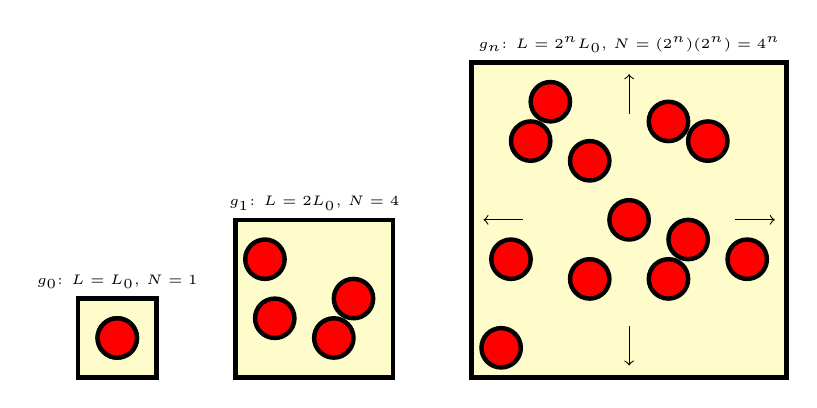
\begin{tikzpicture}
            \draw[black, ultra thick, fill=yellow, fill opacity=.2] (0,0) rectangle (1,1);
            \draw[black, ultra thick, fill=yellow, fill opacity=.2] (2,0) rectangle (4,2);
            \draw[black, ultra thick, fill=yellow, fill opacity=.2] (5,0) rectangle (9,4);
            %\draw[black, ultra thick, fill=yellow, fill opacity=.2] (10,0) rectangle (14,4);
            \draw[<-] (5.15,2) to (5.65,2);
            \draw[->] (7,3.35) to (7,3.85);
            \draw[<-] (7,.15) to (7,.65);
            \draw[->] (8.35,2) to (8.85,2);
            \node[above] at (.5,1) {\tiny $g_0$: $L=L_0$, $N=1$};
            \node[above] at (3,2) {\tiny $g_1$: $L=2L_0$, $N=4$};
            %\node[above] at (7,4) {\tiny $g_2$: $L=4L_0$, $N=8$};
            \node[above] at (7,4) {\tiny $g_n$: $L=2^nL_0$, $N=(2^n)(2^n)=4^n$};

            % Balls!
            \draw[ultra thick, fill=red] (.5,.5) circle [radius=.25];
            % Second box
            \draw[ultra thick, fill=red] (3.25,.5) circle [radius=.25];
            \draw[ultra thick, fill=red] (3.5,1) circle [radius=.25];
            \draw[ultra thick, fill=red] (2.375,1.5) circle [radius=.25];
            \draw[ultra thick, fill=red] (2.5,.75) circle [radius=.25];
            % third
            \draw[ultra thick, fill=red] (5.5,1.5) circle [radius=.25];
            \draw[ultra thick, fill=red] (5.375,.375) circle [radius=.25];
            \draw[ultra thick, fill=red] (6,3.5) circle [radius=.25];
            \draw[ultra thick, fill=red] (7.5,3.25) circle [radius=.25];
            \draw[ultra thick, fill=red] (.5,.5) circle [radius=.25];    
            \draw[ultra thick, fill=red] (7,2) circle [radius=.25];        
            \draw[ultra thick, fill=red] (5.75,3) circle [radius=.25];        
            \draw[ultra thick, fill=red] (6.5,2.75) circle [radius=.25];        
            \draw[ultra thick, fill=red] (8, 3) circle [radius=.25];        
            \draw[ultra thick, fill=red] (7.5,1.25) circle [radius=.25];        
            \draw[ultra thick, fill=red] (7.75,1.75) circle [radius=.25];        
            \draw[ultra thick, fill=red] (8.5,1.5) circle [radius=.25];
            \draw[ultra thick, fill=red] (6.5,1.25) circle [radius=.25];                
     \end{tikzpicture}}
\caption{2-D Demonstration of MC-GRGT doubling method.}
\label{GRTG-demo} 
\end{figure} 

%%%%%% TIKZZZZ %%%%%%


\subsection{Thermodynamic Integration}
\subsubsection{General Process}
Thermodynamic Integration is a unique way to determine the ``excess'' free energy of the system. Using hard sphere Monte-Carlo, we transition from a filling fraction of zero (note that this statement is identical to assuming that the cell begins at infinite temperature, since the total energy does not depend on where the spheres are placed) to a near-close-packed system with filling fraction $\eta_max$, calculating the change in free energy at each step. When we have reached the desired final filling fraction we have found the free energy that was necessary to create that configuration of particles - this is exactly the absolute free energy of the system.\\
\subsubsection{Algorithm}
The hard sphere fluid is simple to work with since its partition function simply counts the number of microstates in the system\cite{valeskethesis}. Since we are calculating the change in free energy as we transition to higher and higher filling fractions, we need only be concerned with finding the ratio of partition functions between each step. Since the hard sphere partition function is a ``counting'' mechanism, we can determine this ratio quite easily using Monte Carlo simulations. Given a starting state (defined by the arrangement of particles and filling fraction) we shrink the volume and intermolecular distances by a somewhat arbitrary scaling factor and then see if the resulting configuration of particles is valid. If the configuration is valid, we accept this is a working move and then return to the original configuration and test another scaling factor. If the resulting configuration is invalid, we count the move as failed and then repeat. The ``golden'' acceptance ratio is fifty percent - when we have found a scaling factor that yields a ratio near the desired value\dots\\

As with the Monte Carlo these simulations are written in $C++$ for efficiency. 

\begin{algorithm}[!b]
\caption{Thermodynamic integration.}
\label{alg:ti}
\begin{alg}
\item Construct cell with desired number of spheres with filling fraction of zero.
\item Move spheres random fractions of a predefined translation distance. \label{alg-ti-move}
\item Repeat step \ref{alg-ti-move} for [desired number of iterations before small cell check].
\item After [desired number of iterations], check the ``small cell'' by shrinking the volume and checking whether or not the configuration is still valid.
\item If configuration is still valid, valid checks ++.
\item If configuration is invalid, failed checks ++. \label{alg-ti-move-end}
\item Repeat steps \ref{alg-ti-move} - \ref{alg-ti-move-end} until desired iterations reached.

\end{alg}      
\end{algorithm}  

\ignore{Should I detail the algorithm itself and string simulations together or consider the entire process $\eta=0\rightarrow\eta_max$ to be the algorithm?}



\ignore{is the distinction between infinite case and regular necessary? we always use infinite...}

\begin{figure} \centering
\resizebox{.75\textwidth}{!}{
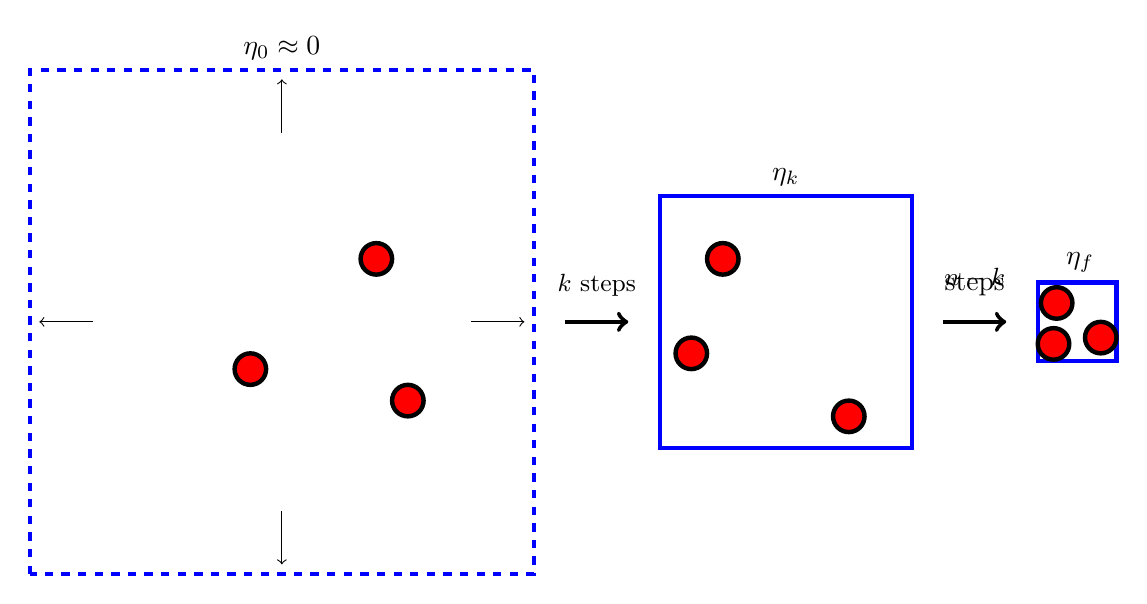
\begin{tikzpicture}[scale=.8,  auto]
\draw[blue, ultra thick] (10,3) rectangle (14,7);
\draw[blue, ultra thick, dashed] (0,1) rectangle (8,9);
\draw[blue, ultra thick] (16,4.375) rectangle (17.25,5.625);
\draw[->] (4,8) to (4, 8.85);
\draw[->] (7,5) to (7.85, 5);
\draw[->] (1,5) to (.15, 5);
\draw[->] (4,2) to (4, 1.15);
\draw[ultra thick, ->] (8.5,5) to (9.5,5);
\node [above] at (9,5.25) {\small $k$ steps};
\draw[ultra thick, ->] (14.5,5) to (15.5,5);
\node[align=center] [above] at (15, 5.25) {\small $n-k$ \\[-1em] steps};
\draw[ultra thick, fill=red] (3.5,4.25) circle [radius=.25];
\draw[ultra thick, fill=red] (6,3.75) circle [radius=.25];
\draw[ultra thick, fill=red] (5.5,6) circle [radius=.25];
\draw[ultra thick, fill=red] (10.5,4.5) circle [radius=.25];
\draw[ultra thick, fill=red] (13,3.5) circle [radius=.25];
\draw[ultra thick, fill=red] (11,6) circle [radius=.25];
\draw[ultra thick, fill=red] (16.3,5.3) circle [radius=.25];
\draw[ultra thick, fill=red] (17,4.75) circle [radius=.25];
\draw[ultra thick, fill=red] (16.25,4.65) circle [radius=.25];
\node [above] at
 (4,9) {$\eta_0 \approx 0$};
\node [above] at (12,7) {$\eta_k$};
\node [above] at (16.675,5.625) {$\eta_f$}; 
\end{tikzpicture}}
\caption{Demonstration of filling fraction increase during thermodynamic integration from $\eta=0$ to $\eta=\eta_f=\eta_{max}$.}
\end{figure}

\subsubsection{Carnahan-Starling Equation of State}
In order to determine the filling fraction step size during thermodynamic integration we must find changes in filling fraction that yield a suitably-sized change in the system's absolute free energy. To do this we use the Carnahan-Starling equation of state, shown in Eq.~\ref{C-S-eq}.
\begin{align}
    F(\eta) &= \frac{4\eta - 3\eta^2}{(1-\eta)^2}   
    \label{C-S-eq}  
\end{align} 
where $\eta$ is the filling fraction. Combining Eq.~\ref{C-S-eq} with a simple bisection method allows for control of the filling fraction step size given a desired change in free energy. We determined that steps yielding an approximate change in specific absolute free energy of $\Delta F^{abs}/NT = \ln(2)$ through trial and error - smaller step sizes unnecessarily increased simulation time and larger step sizes tended to shrink too quickly causing the simulation to miss relevant states in the system. 

\ignore{NB: is there a more physical reason we chose this filling fraction increase?}

\subsection{Data Storage}
All simulation output is saved in text files for plotting and visualization ease. The question of organization becomes important with this amount of files being generated. Each different system simulation (length $L = \sqrt2 \sigma, 5,10$) has data regarding each doubling regime ($i=0,1,2,3?$) and each doubling regime contains data for each possible sphere count ($N=1,2,3\dots N_{max}$, where $N_{max}$ is typically limited by maximal sphere packing of $N_{max}/L^3\approx.741$). The file structure mirrors the above symmetry: 
\begin{align*}
                &\rightarrow \text{i=0} &\rightarrow \text{N=0}\\
                & &\rightarrow \text{N=1}\\
                && \vdots\\
\text{System} & \rightarrow \text{i=1} &\rightarrow \text{N=0}\\
                && \rightarrow \text{N=1}\\
                &&\vdots\\
                &\rightarrow \text{i=2} &\rightarrow \text{N=0}\\
                && \rightarrow \text{N=1}\\
                &&\vdots\\
\end{align*}
Each sphere count subfolder contains a single text file from TMMC output and another subfolder where all of the Thermodynamic Integration output is stored. Each Thermodynamic Integration simulation outputs a single text file upon completion of each filling fraction step. On average, a single TI calculation requires approximately $175$ steps. \\
This structure was chosen both for elegant parallelism and for plotting accessibility. 

\subsection{Calculating the Absolute Change in Free Energy}
It is straightforward the compute a Helmholtz free energy through the Monte-Carlo simulations; the difficulty in this method lies in computing the correct free energy. TMMC, as mentioned previously, yields a free energy accurate only up to a unknown constant. Since we need to add up changes in free energy across multiple simulations, we need each calculated free energy to be ``absolute'' - that is, we must eliminate this unknown constant. \\

At infinite temperature, the square well fluid behaves exactly as the hard sphere. The correct inclusion, then, is to enforce that the free energy calculated via TMMC at $T=\infty$ is equal to the free energy calculated through thermodynamic integration. We do this by exploiting the infinite temperature behavior of the canonical ensemble:
\begin{align}
    Z(T=\infty) &= \left.\sum_{i=0}^{\text{\tiny Energies}} D(E) e^{-\beta E}\right|_{\beta = 0}\\
    &= \sum_{i=0}^{\text{\tiny Energies}} D(E)\\
    &= \#\text{~states}
\end{align}

\ignore{NB: cough cough the HS energy probs wrong}
The partition function now calculates the total number of states in the system which we expected due to the equipartition theorem. The hard sphere free energy [more] 




\section{Results}
An important remaining question is whether there is a preferred choice of minimum cell length. Physically we would [might?] expect that there is some dominant minimum fluctuation in the bulk cell - this would then lend a natural decision for the minimum cell length $\lambda_0$. Unfortunately we do not know this {\it a priori}, so we are reduced to guessing. Using the coupling procedure outlined previously, we calculated changes in free energy up to the $n^{\text{th}}$ doubling regime for several different cell lengths. We are primarily concerned with the ``scrunched'' case where the cell length is $\sqrt2\sigma$.

Figures ~\ref{F-T} and ~\ref{F-eta} show preliminary free energy calculations.
\begin{figure}[H]
\centering
    \includegraphics[width=.75\textwidth]{ww130-L03-i1_F-T.pdf}
    \caption{Preliminary results for absolute specific free energy as a function of temperature with each quantity scaled by well depth $\epsilon$. The vertical line at $T/\epsilon = 0.3$ is the lowest temperature at which our statistics are trustworthy.}
    \label{F-T}
\end{figure}
\begin{figure}
\centering
    \includegraphics[width=.75\textwidth]{ww130-L03-F_i1_fixed_i.pdf}
    \caption{Preliminary results for free energy as a function of density.}
    \label{F-eta}
\end{figure}

\subsection{Primitive Cell}
The ``scrunched'' system allows exactly four spheres to be packed -- at maximal filling fraction $\eta_{max} = \approx .741$ -- in the original non-doubled cell. This case corresponds to the unit cell a face-centered cubic lattice, the simplest sphere packing possible. We chose to focus on the scrunched case for two reasons. Firstly, if any physical length of the system is likely to be the correct choice for minimum fluctuation length 

\subsubsection{Seed Disparity}
Because of the random/psuedorandom nature of Monte-Carlo sampling, we tested over many different initial sphere placements (``seeds'') to see if there was consistent agreement. 
\subsection{Other Cells?}
In addition to the ``scrunched'' primitive cell, we tested [hopefully one or two] other minimum correlation lengths corresponding to other natural parameters in the system.

%%%%%%%%%%%%%%%%%%%%%%%%%%%%%%%%%%%%%%%%%%%%%%%%%%%%%%%%%%%%%%%
%                       Discussion                            %
%%%%%%%%%%%%%%%%%%%%%%%%%%%%%%%%%%%%%%%%%%%%%%%%%%%%%%%%%%%%%%%

\section{Discussion}
If the decomposition procedure outlined previously proves successful, the absolute free energy yielded by this renormalization method ought to agree with the free energy yielded from other accepted theories. [more]
\subsection{Change in Free Energy Over Multiple Regimes}
[more]
\subsection{Comparison With A Modified Statistical Associating Fluid Theory}
[more]

%%%%%%%%%%%%%%%%%%%%%%%%%%%%%%%%%%%%%%%%%%%%%%%%%%%%%%%%%%%%%%%%%%
%                             CONCLUSION                         %
%%%%%%%%%%%%%%%%%%%%%%%%%%%%%%%%%%%%%%%%%%%%%%%%%%%%%%%%%%%%%%%%%%


\section{Conclusion}


\subsection{Future Research}
There are many other models that GRGT might be applicable to, such as the soft-sphere liquid or soft polyhedra.
%\bibliographystyle{plain}
\bibliography{Thesis}
\end{document}